\subsection{Medición de la resistencia interna de un osciloscopio} \label{sec:resistencia de osc}

\paragraph{}
En esta sección se determinó la resistencia interna de un osciloscopio. Para esto, se armó el circuito de la figura \ref{fig:esq_osciloscopio}. Se utilizó un amperímetro para registrar la corriente del circuito, conectado en serie para que su resistencia sea despreciable con respecto al resto, y se utilizó un voltímetro como resistencia, conectada en paralelo con el osciloscopio.

\begin{figure}[H]
    \centering
    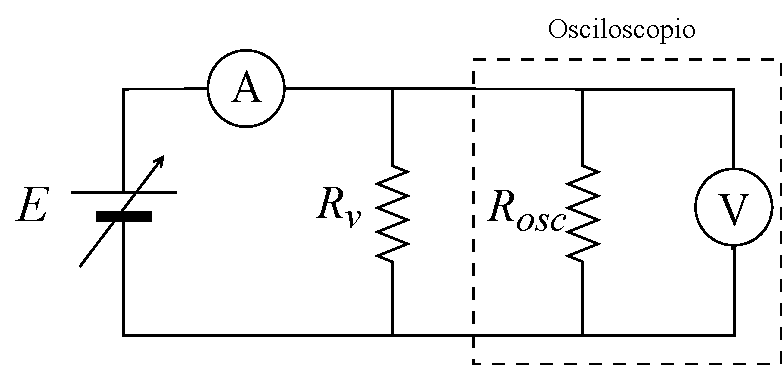
\includegraphics[width = 0.6\linewidth]{Esquemas/Osciloscopio.pdf}
    \caption{Esquema de un circuito eléctrico dotado de una fuente de voltaje variable $E$, un amperímetro, una resistencia $R_v$ y un osciloscopio. El osciloscopio está modelado como un voltímetro con su respectiva resistencia}
    \label{fig:esq_osciloscopio}
\end{figure}

\paragraph{}
Se registraron la corriente y la diferencia de potencial con el amperímetro y osciloscopio respectivamente, y se realizó un ajuste a partir de la ecuación \ref{eqn:ley de ohm}, utilizando la resistencia equivalente obtenida con la ecuación \ref{eqn: en paralelo}. El gráfico de este ajuste se puede observar en la figura \ref{fig:fig_osciloscopio}.

\begin{figure}[H]
    \centering
    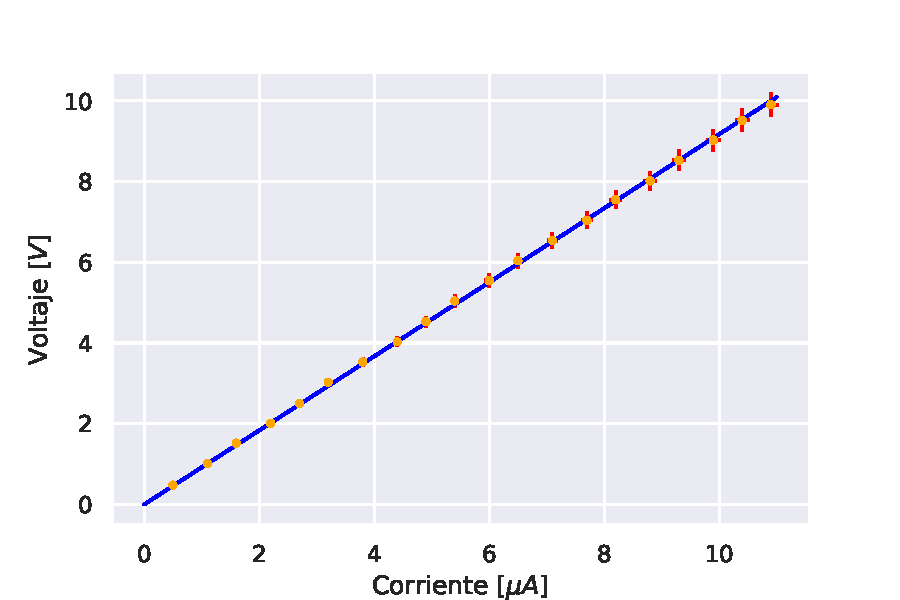
\includegraphics[width = 0.65\linewidth]{figuras/resistencia osc.pdf}
    \caption{Ajuste lineal que muestra la relación entre la caída de potencial y la corriente. De esta relación se puede obtener $R_{osc}$}
    \label{fig:fig_osciloscopio}
\end{figure}

\paragraph{}
Utilizando el valor de resistencia del voltímetro calculado en la sección \ref{sec:resistencia de volt} y la pendiente dada por el ajuste, se encontró que la resistencia interna del osciloscopio es de  $R_{osc}=(1,009 \pm 0,002)$ M$\Omega$. Este resultado es consistente con el valor esperado para un voltímetro, que se encuentra en el orden de los M$\Omega$.
